\chapter{US labor market}
\label{chap:labor}

In this chapter I examine the US labor market, where the two sided logit model is
originally developed for. Check the results of our model against real data and
look at the fit.

\begin{figure}[!ht]
  \centering
  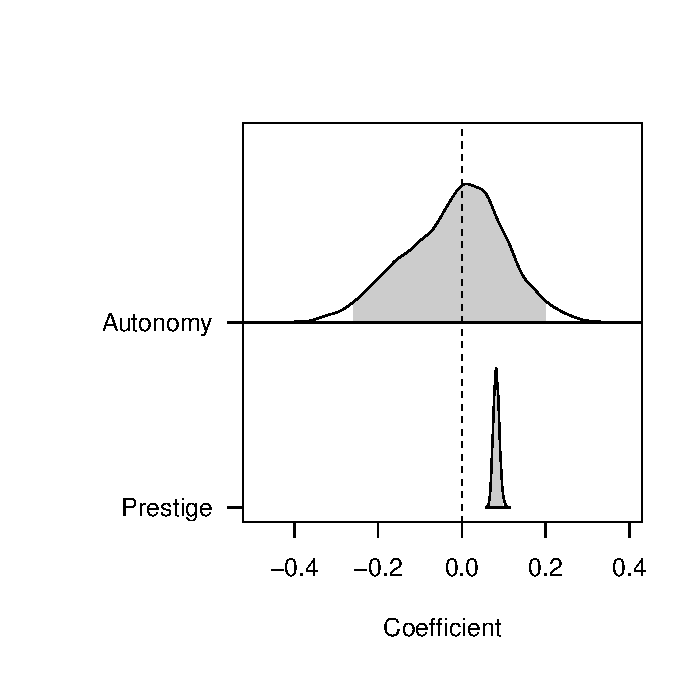
\includegraphics[width=0.75\textwidth,keepaspectratio]{../figure/labor_occ5_alpha}
  \caption[Workers' preference in the US labor market.]{Preference of workers for firms' characteristics. The density plot and the
    shaded region show the posterior distribution and the 95\% credible interval
    after burn-in. While prestige is highly valued by workers, autonomy seems to
    be less importance.}
  \label{fig:labor_occ5_alpha}
\end{figure}

\begin{figure}[!ht]
  \centering
  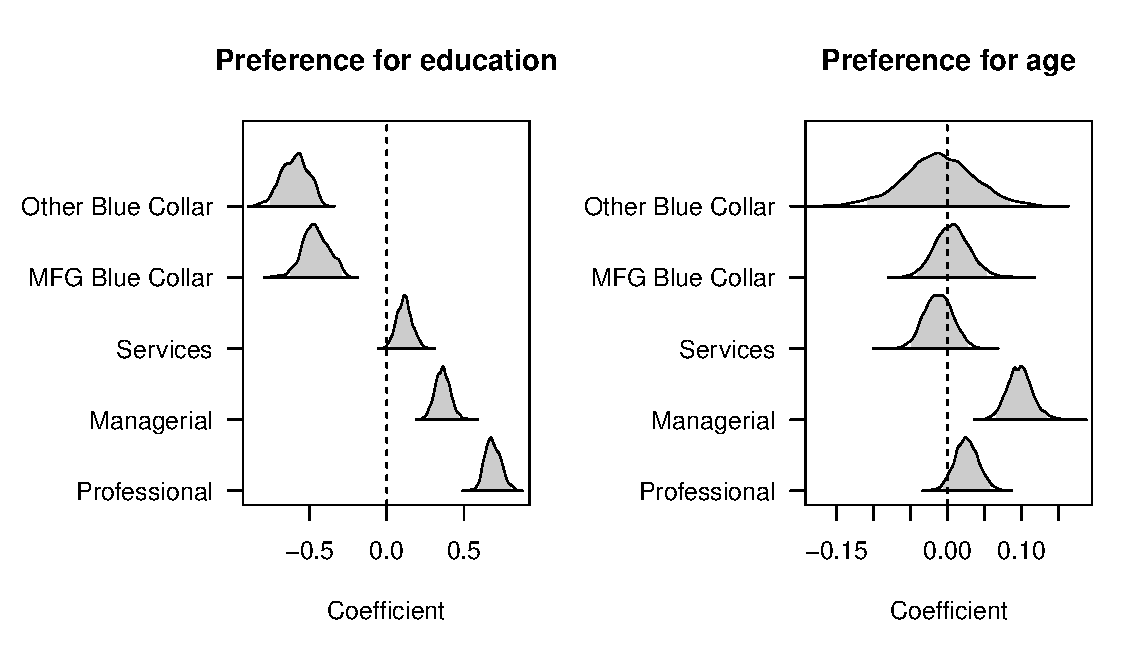
\includegraphics[width=\textwidth,keepaspectratio]{../figure/labor_occ5_beta_educ_age}
  \caption[Firms' preference in the US labor market]{Preference of firms for workers' education and
    age. Professional and managerial firms have a strong and positive preference
  for highly educated workers. While most firms do not highly value older workers,
  except managerial firm stands out in their preference for age (likely as a
  proxy for experience).}
  \label{fig:labor_occ5_beta_educ_age}
\end{figure}

\begin{figure}[!ht]
  \centering 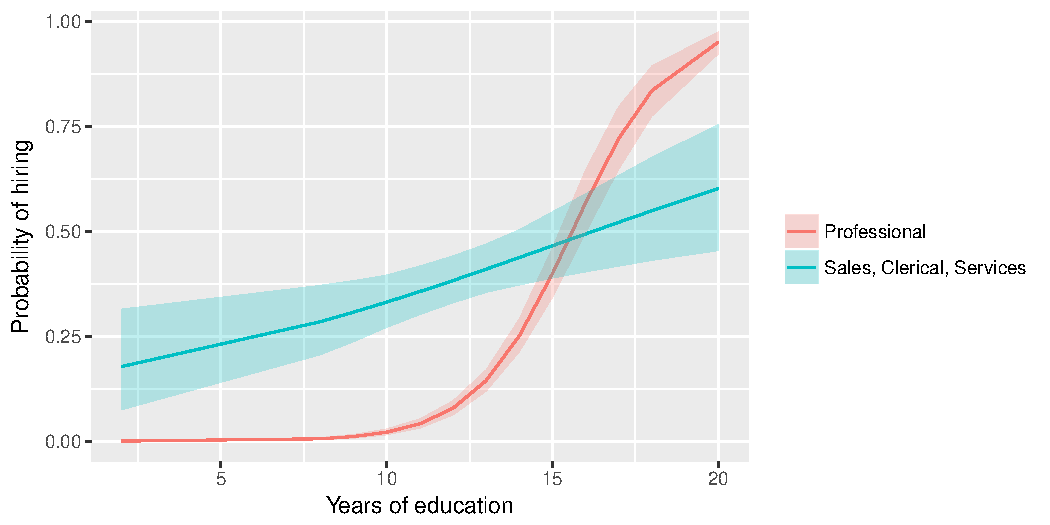
\includegraphics[width=\textwidth,keepaspectratio]{../figure/labor_occ5_educ_effect_on_hiring}
  \caption[The effect of education on the probability of a worker being hired in
  the US labor market.]{The
    effect of education on the probability of a worker being hired into a professional
    and a services job.}
  \label{fig:labor_occ5_educ_effect_on_hiring}
\end{figure}

\begin{figure}[!ht]
  \centering
  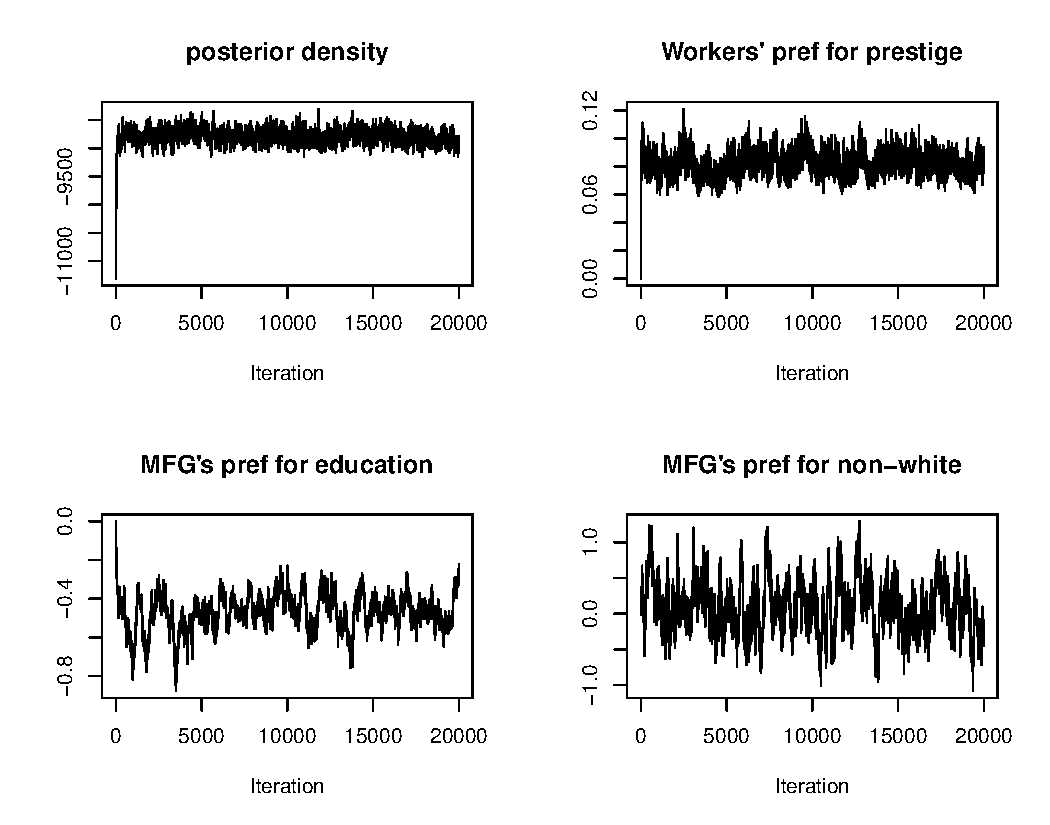
\includegraphics[width=\textwidth,keepaspectratio]{../figure/labor_occ5_misc_traceplots}
  \caption[Parameter traceplots]{Trace plots of the posterior density and
    parameter samples, showing quick convergence.}
  \label{fig:labor_occ5_misc_traceplots}
\end{figure}

%%% Local Variables:
%%% mode: latex
%%% TeX-master: "AnhLe_dissertation.tex"
%%% End: